\section{Testing methods}
A number of algorithms were compared on a set of standard tests to compare the performance:

\begin{itemize}
	\item SISR
	\item SISR FL(5)
	\item RB-SISR FL(5)
	\item MCMC
	\item MCMC FL(5)
	\item RB-MCMC FL(5)
	\item PDAF
	\item JPDAF
\end{itemize}

where FL(N) indicates fixed lag with a window length of N. The test set consisted of:

\begin{enumerate}
	\item 5 widely-spaced targets
	\item 5 widely-spaced targets, high clutter and missed detection rate
	\item 5 widely-spaced targets, high observation noise covariance
	\item 5 closely-spaced targets
\end{enumerate}

Each scenario lasted for 50 time steps. Each was tested using both the linear and bearing-range observation models. Each combination was run with 10 different random seeds. An example of each is shown in figures~\ref{fig:EgScen1} to~\ref{fig:EgScen4}.

\begin{figure}%
\subfigure[state]{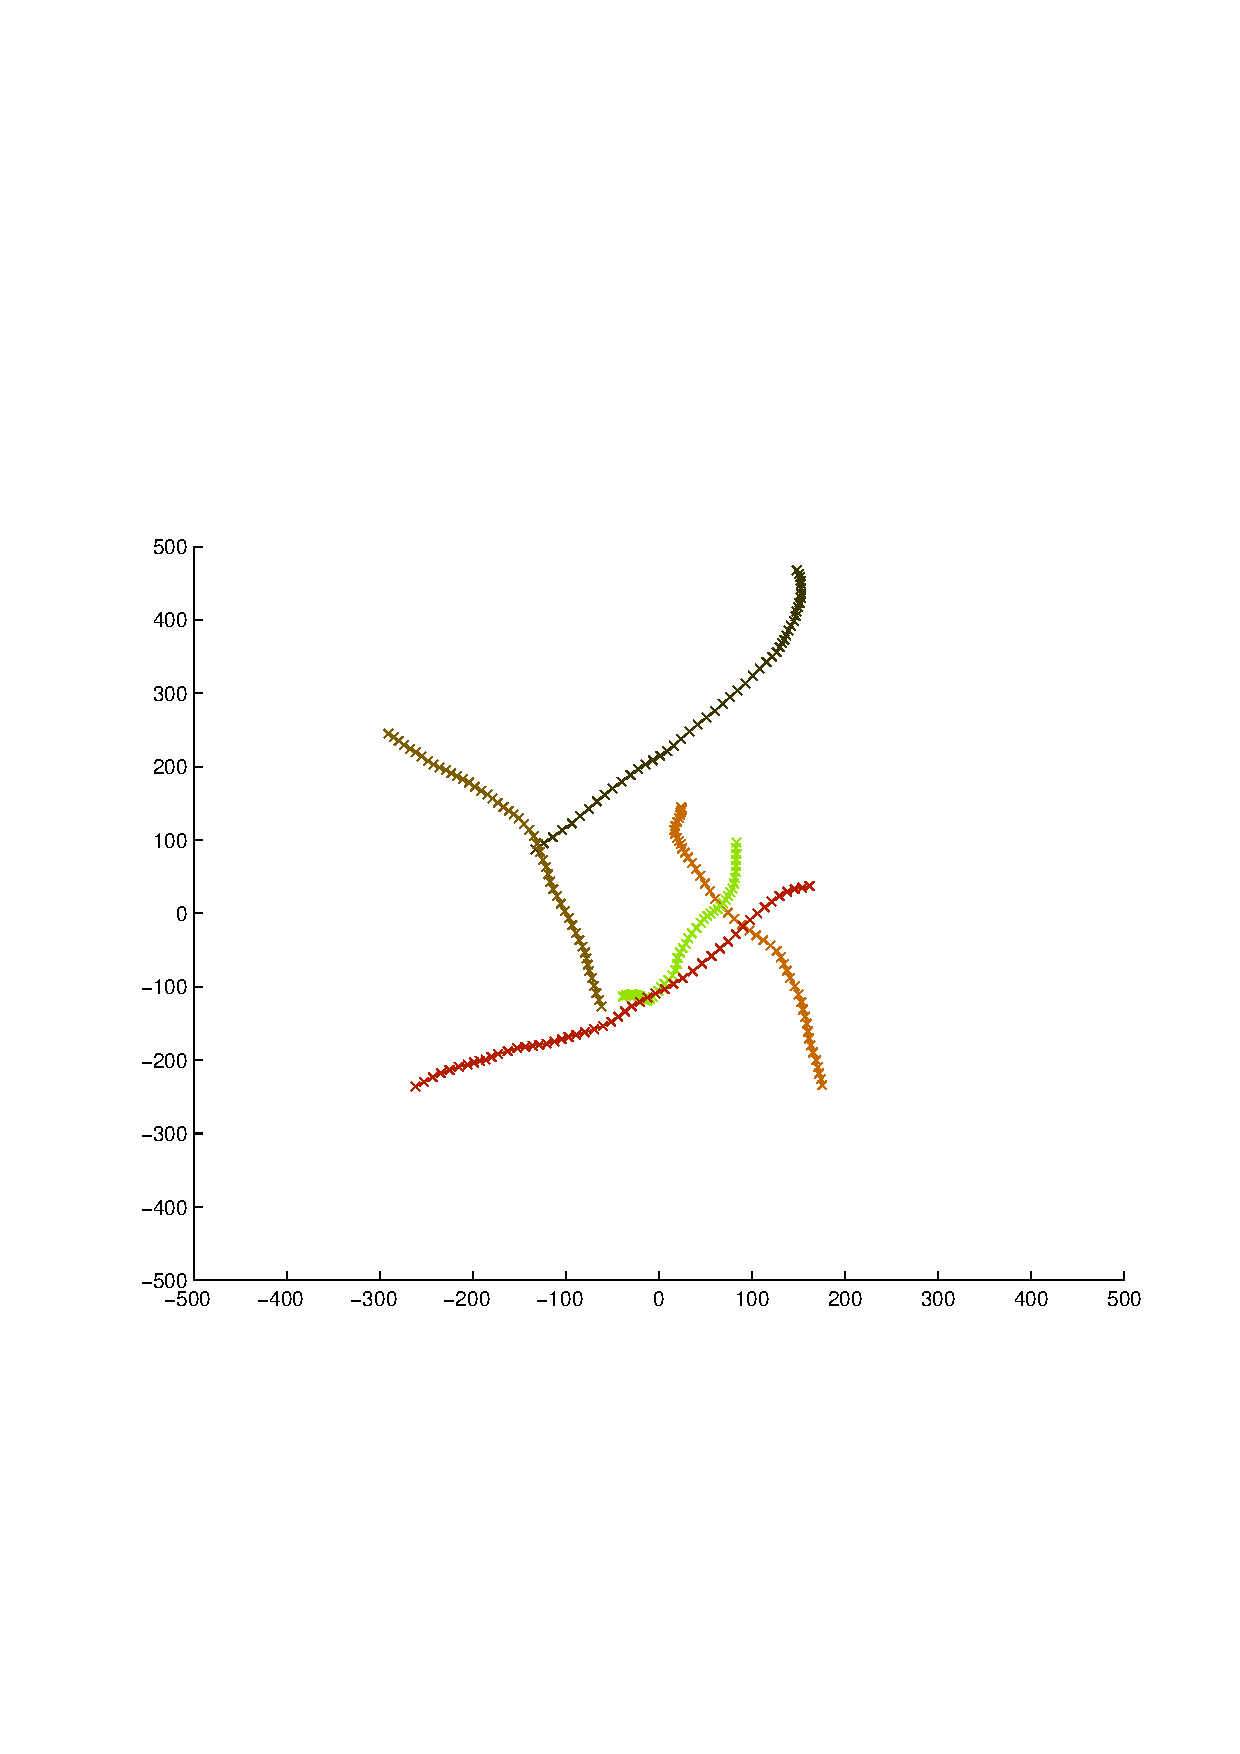
\includegraphics[width=0.3\columnwidth]{results_wide_low_state.pdf}}
\subfigure[linear observations]{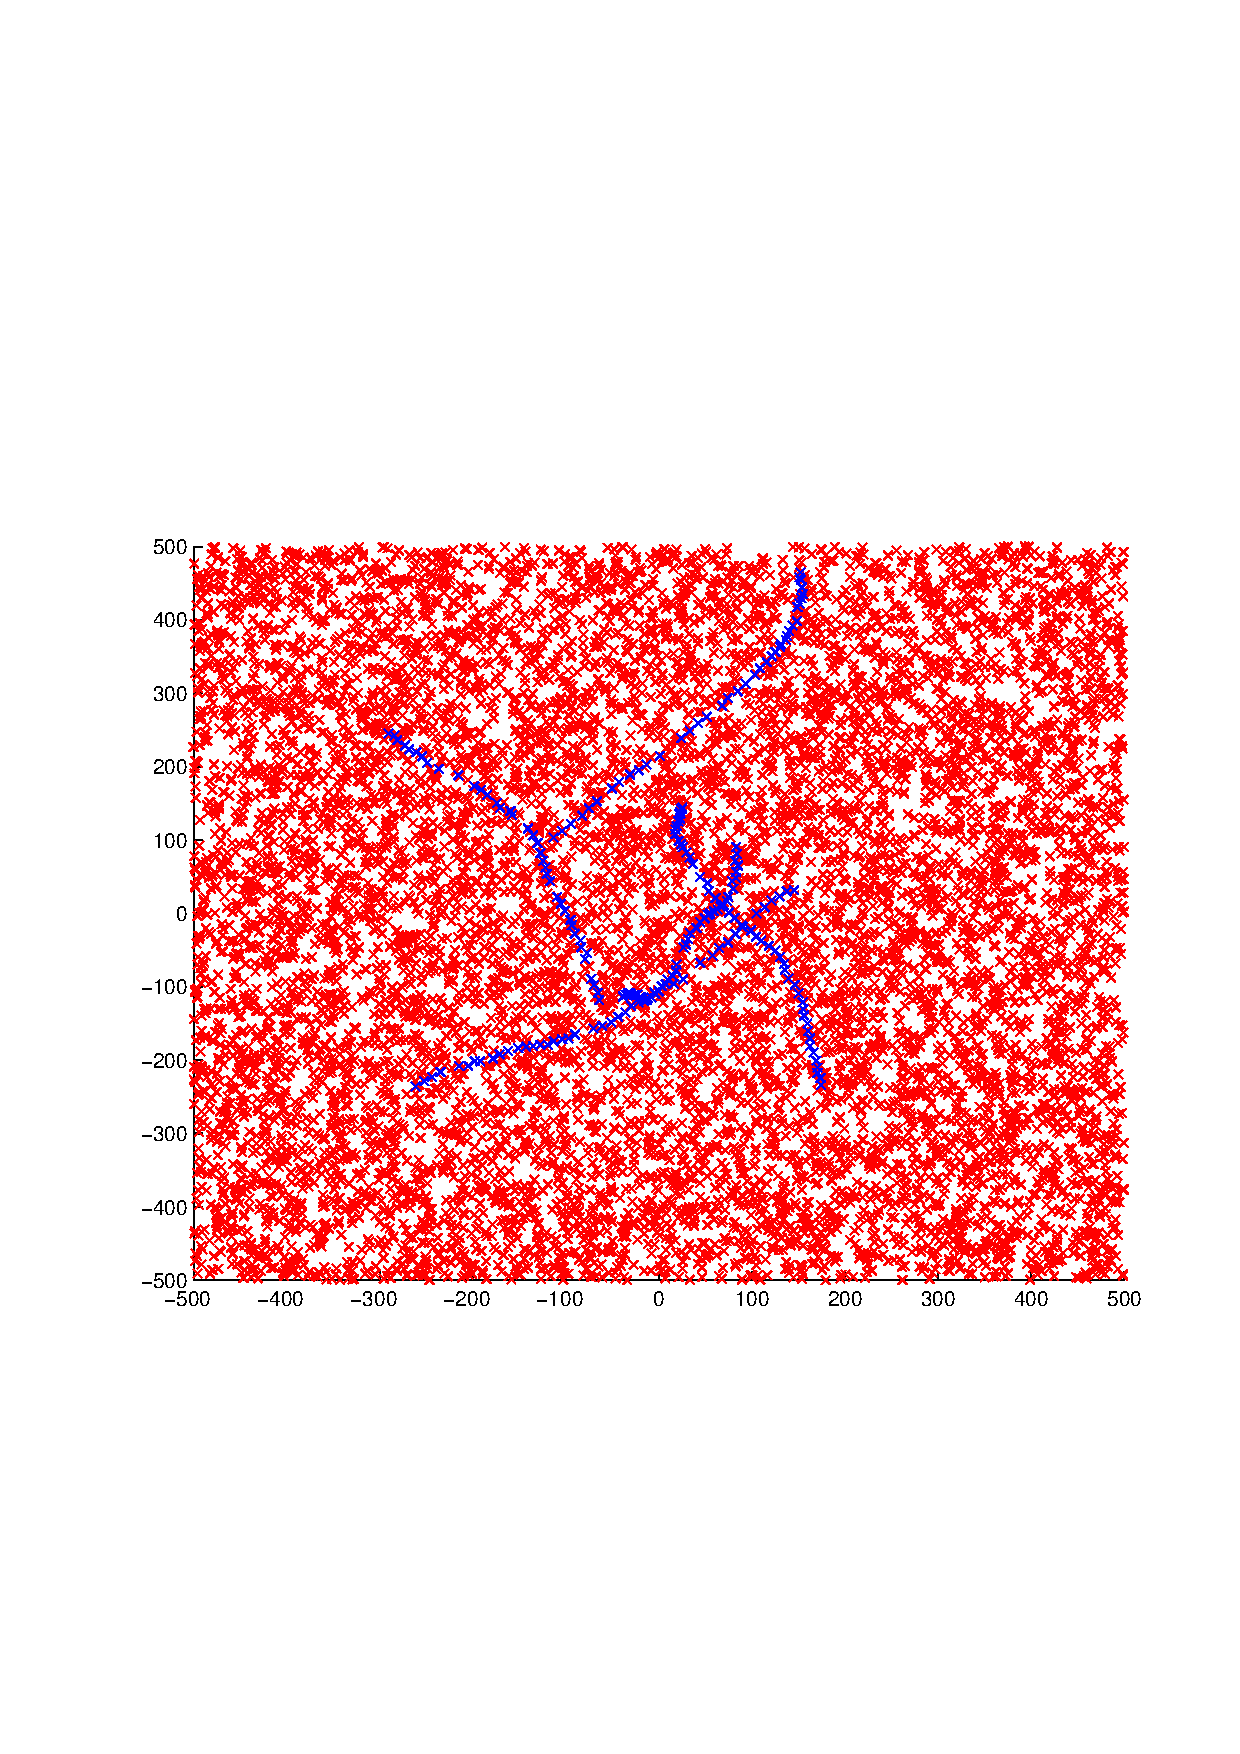
\includegraphics[width=0.3\columnwidth]{results_wide_low_lGobs.pdf}}
\subfigure[bearing-range observations]{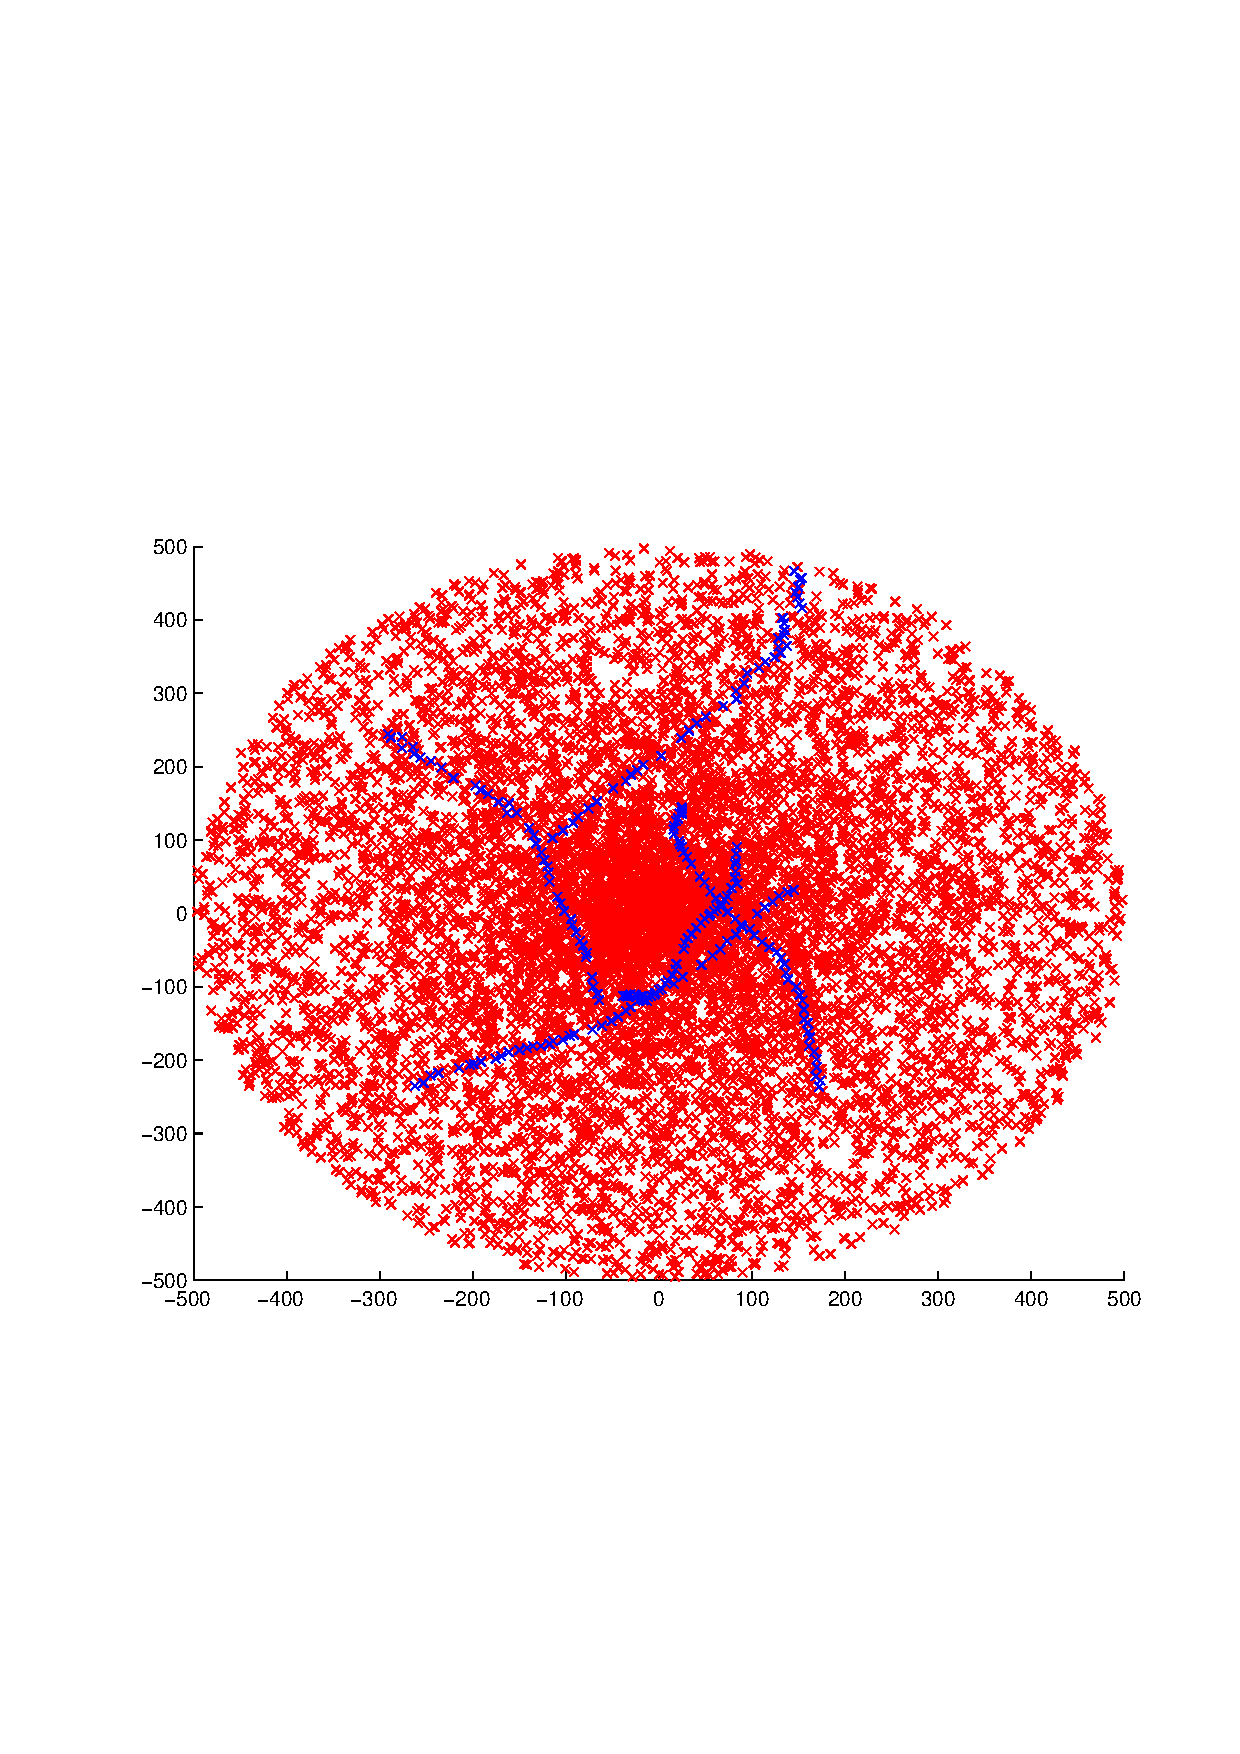
\includegraphics[width=0.3\columnwidth]{results_wide_low_brobs.pdf}}
\caption{Case 1}%
\label{fig:EgScen1}%
\end{figure}
\begin{figure}%
\subfigure[state]{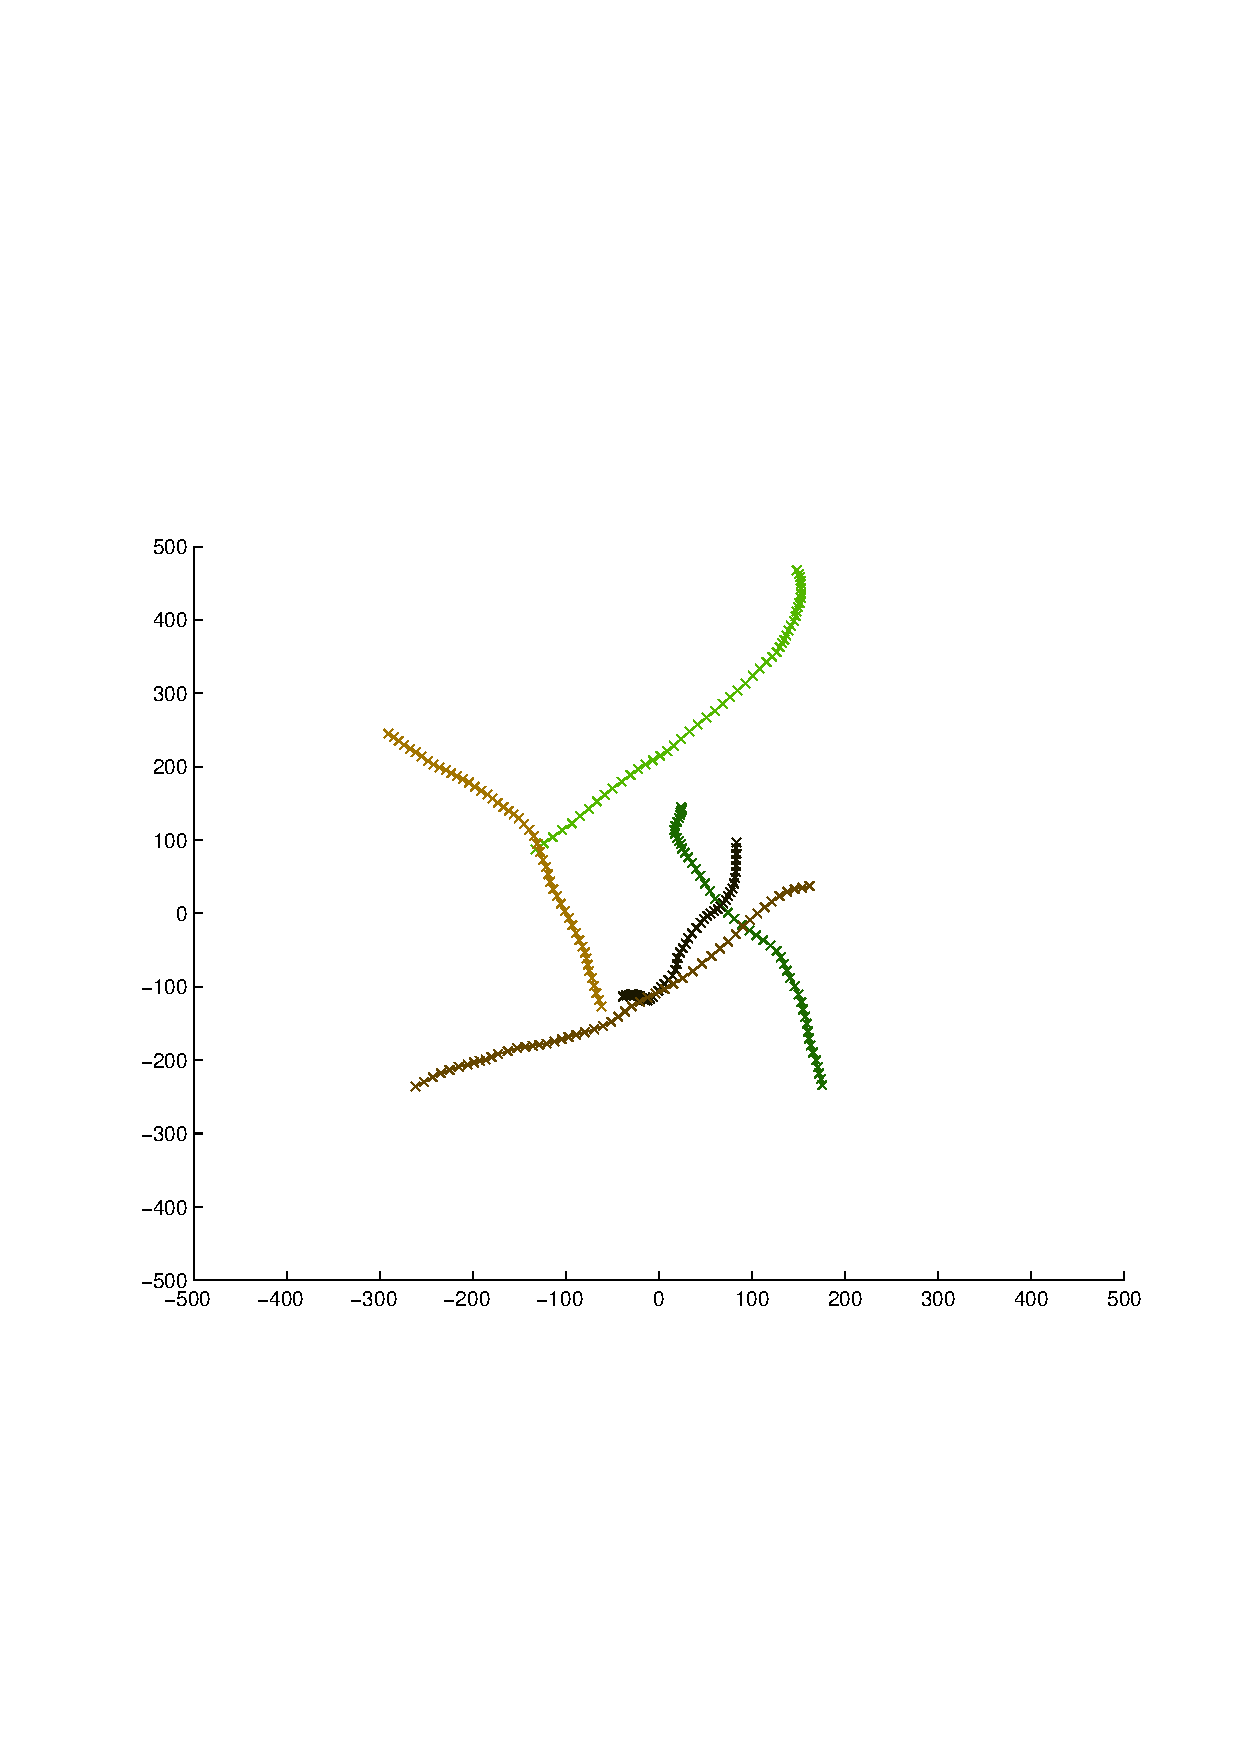
\includegraphics[width=0.3\columnwidth]{results_wide_high_state.pdf}}
\subfigure[linear observations]{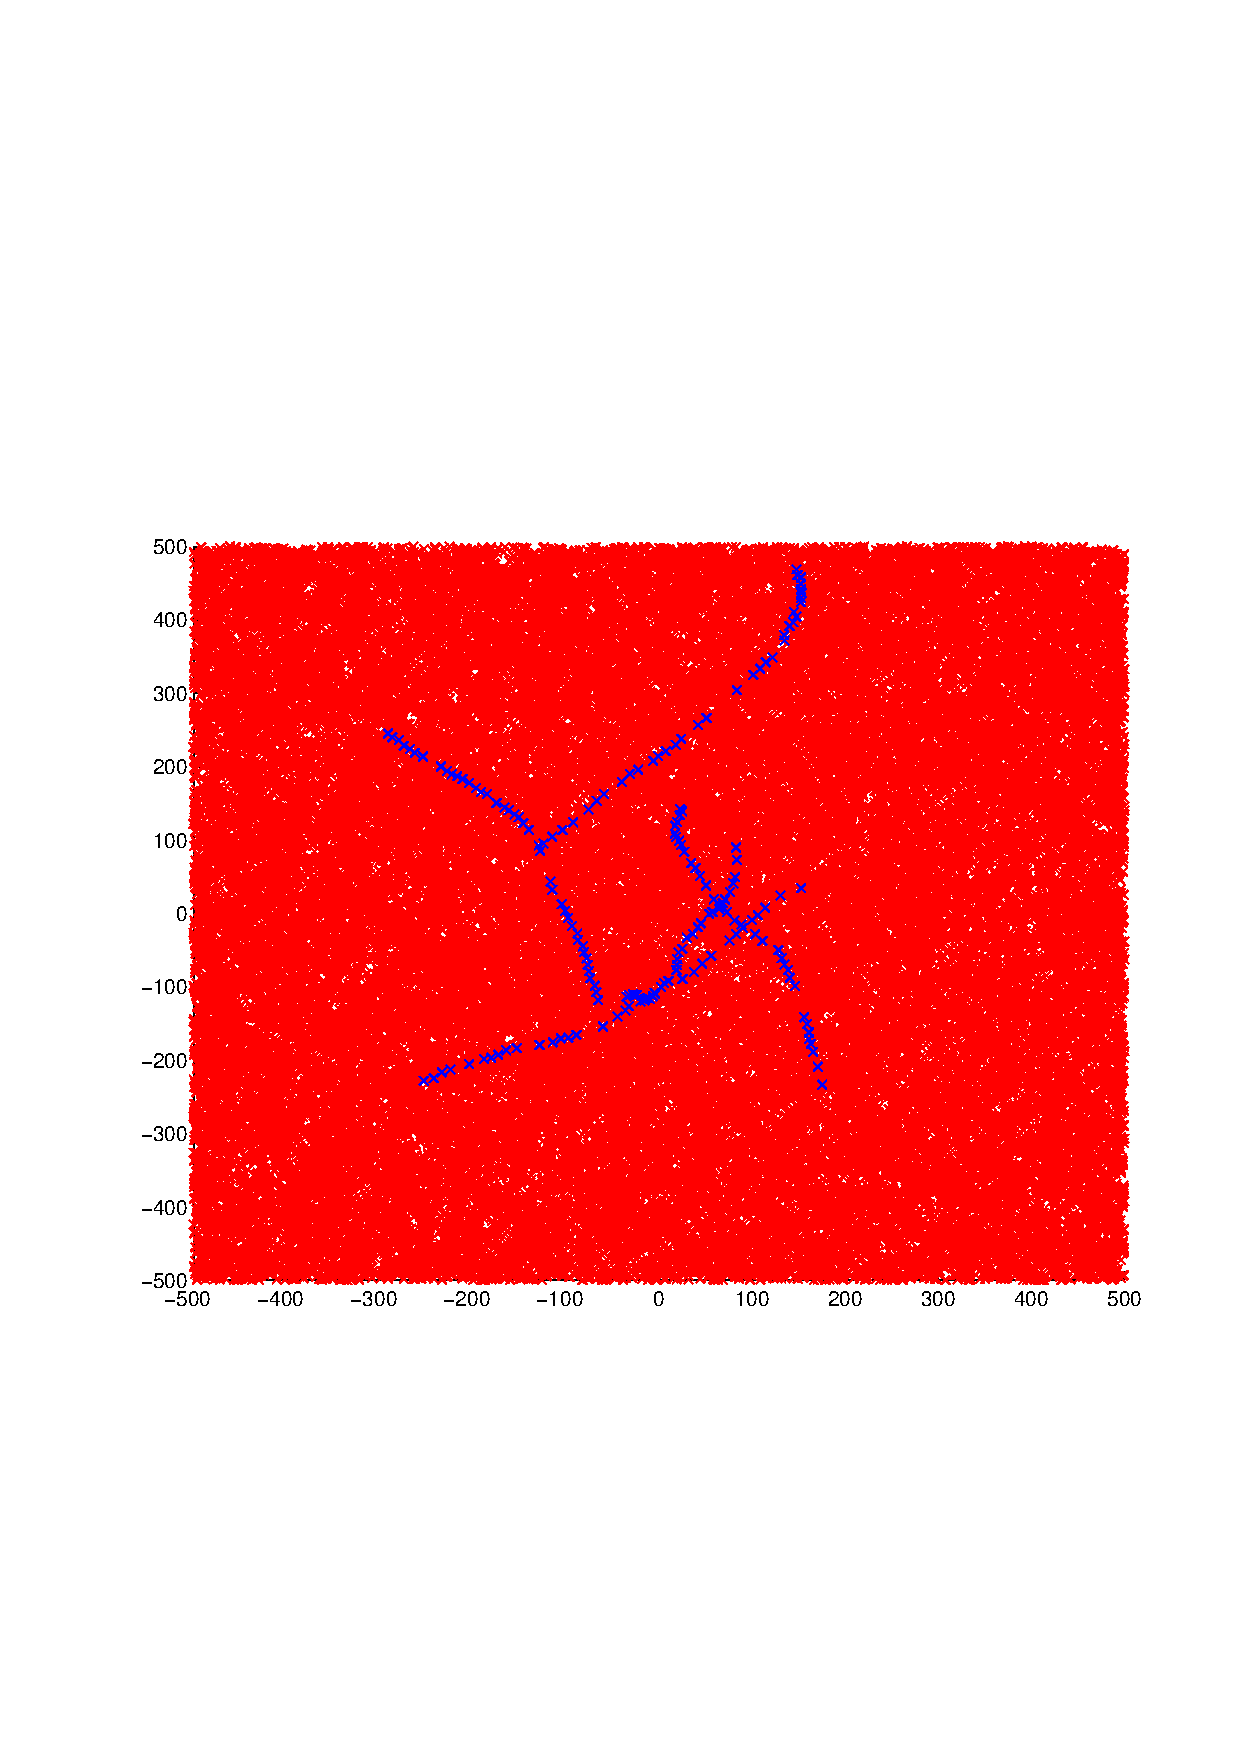
\includegraphics[width=0.3\columnwidth]{results_wide_high_lGobs.pdf}}
\subfigure[bearing-range observations]{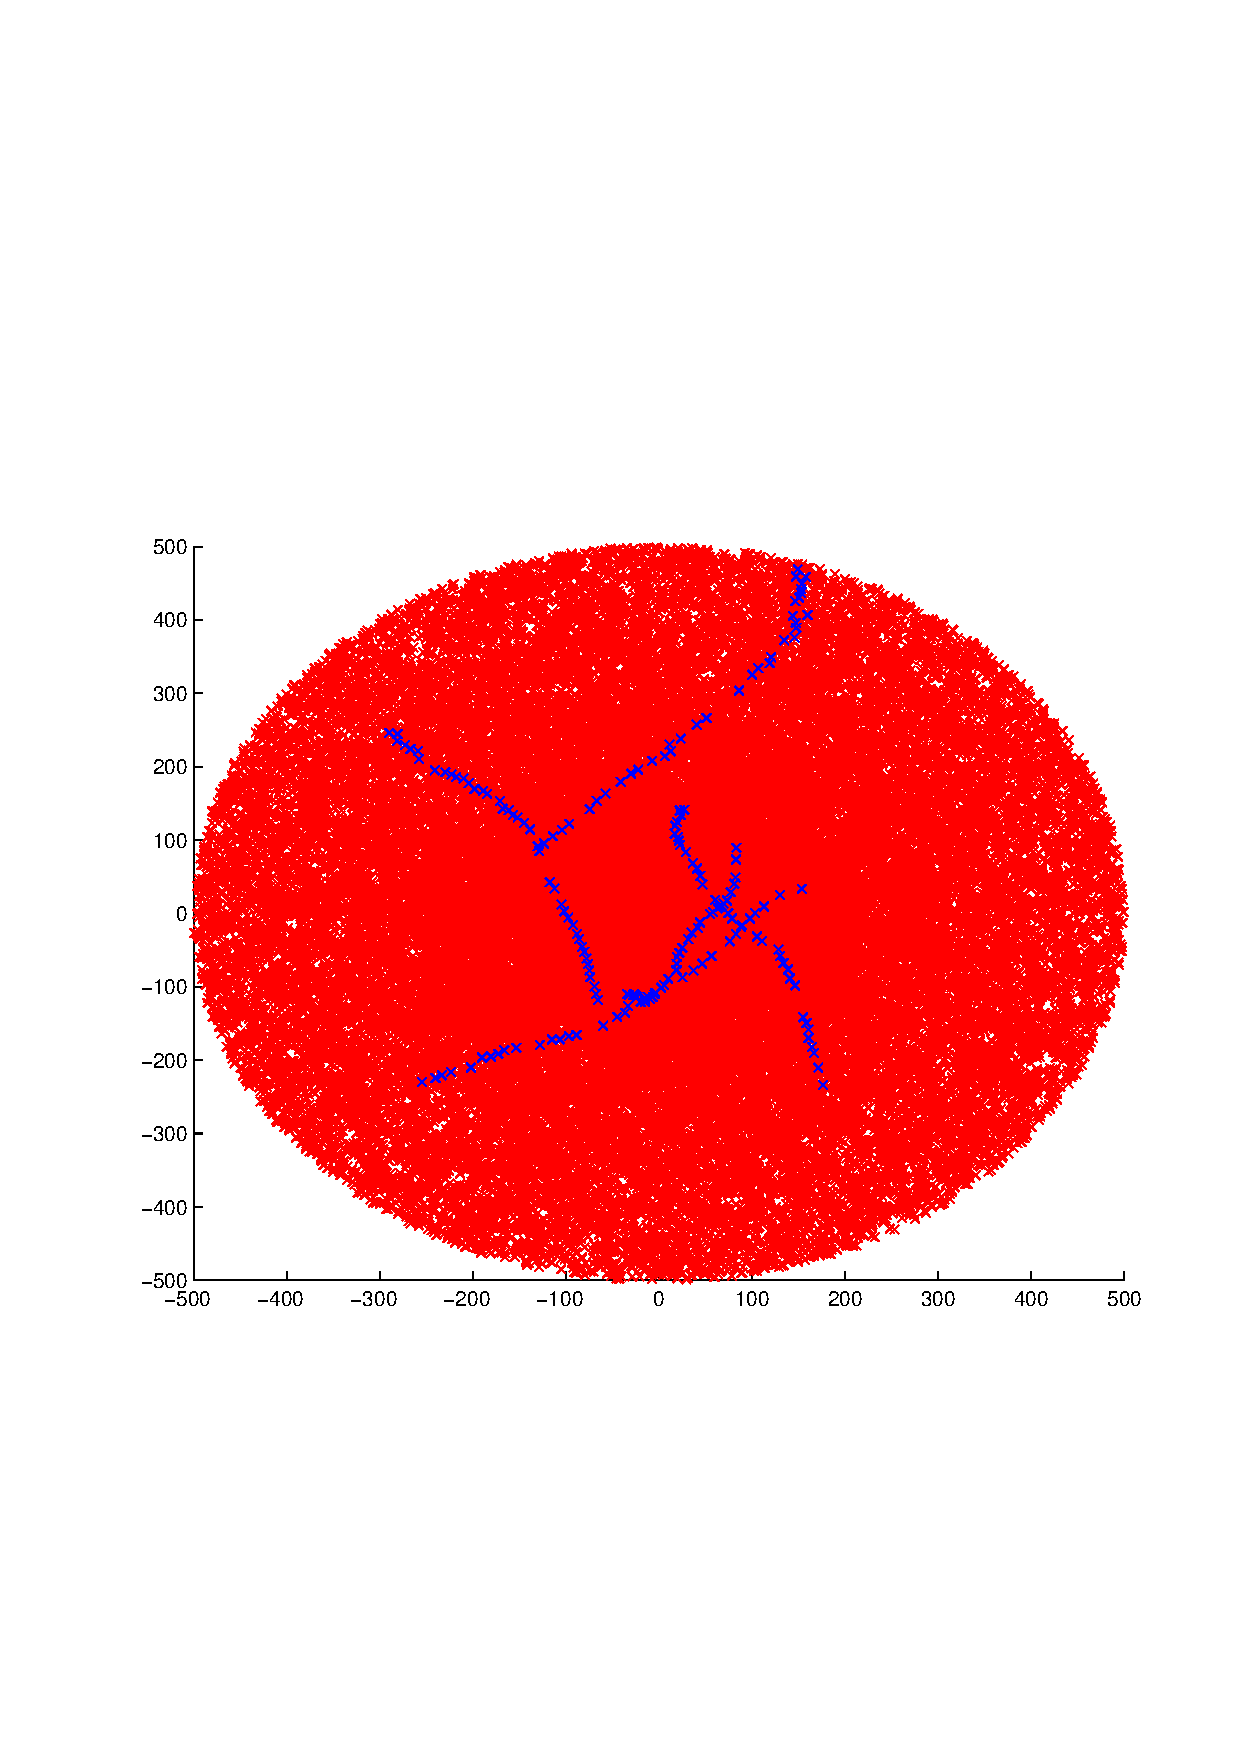
\includegraphics[width=0.3\columnwidth]{results_wide_high_brobs.pdf}}
\caption{Case 2}%
\label{fig:EgScen2}%
\end{figure}
\begin{figure}%
\subfigure[state]{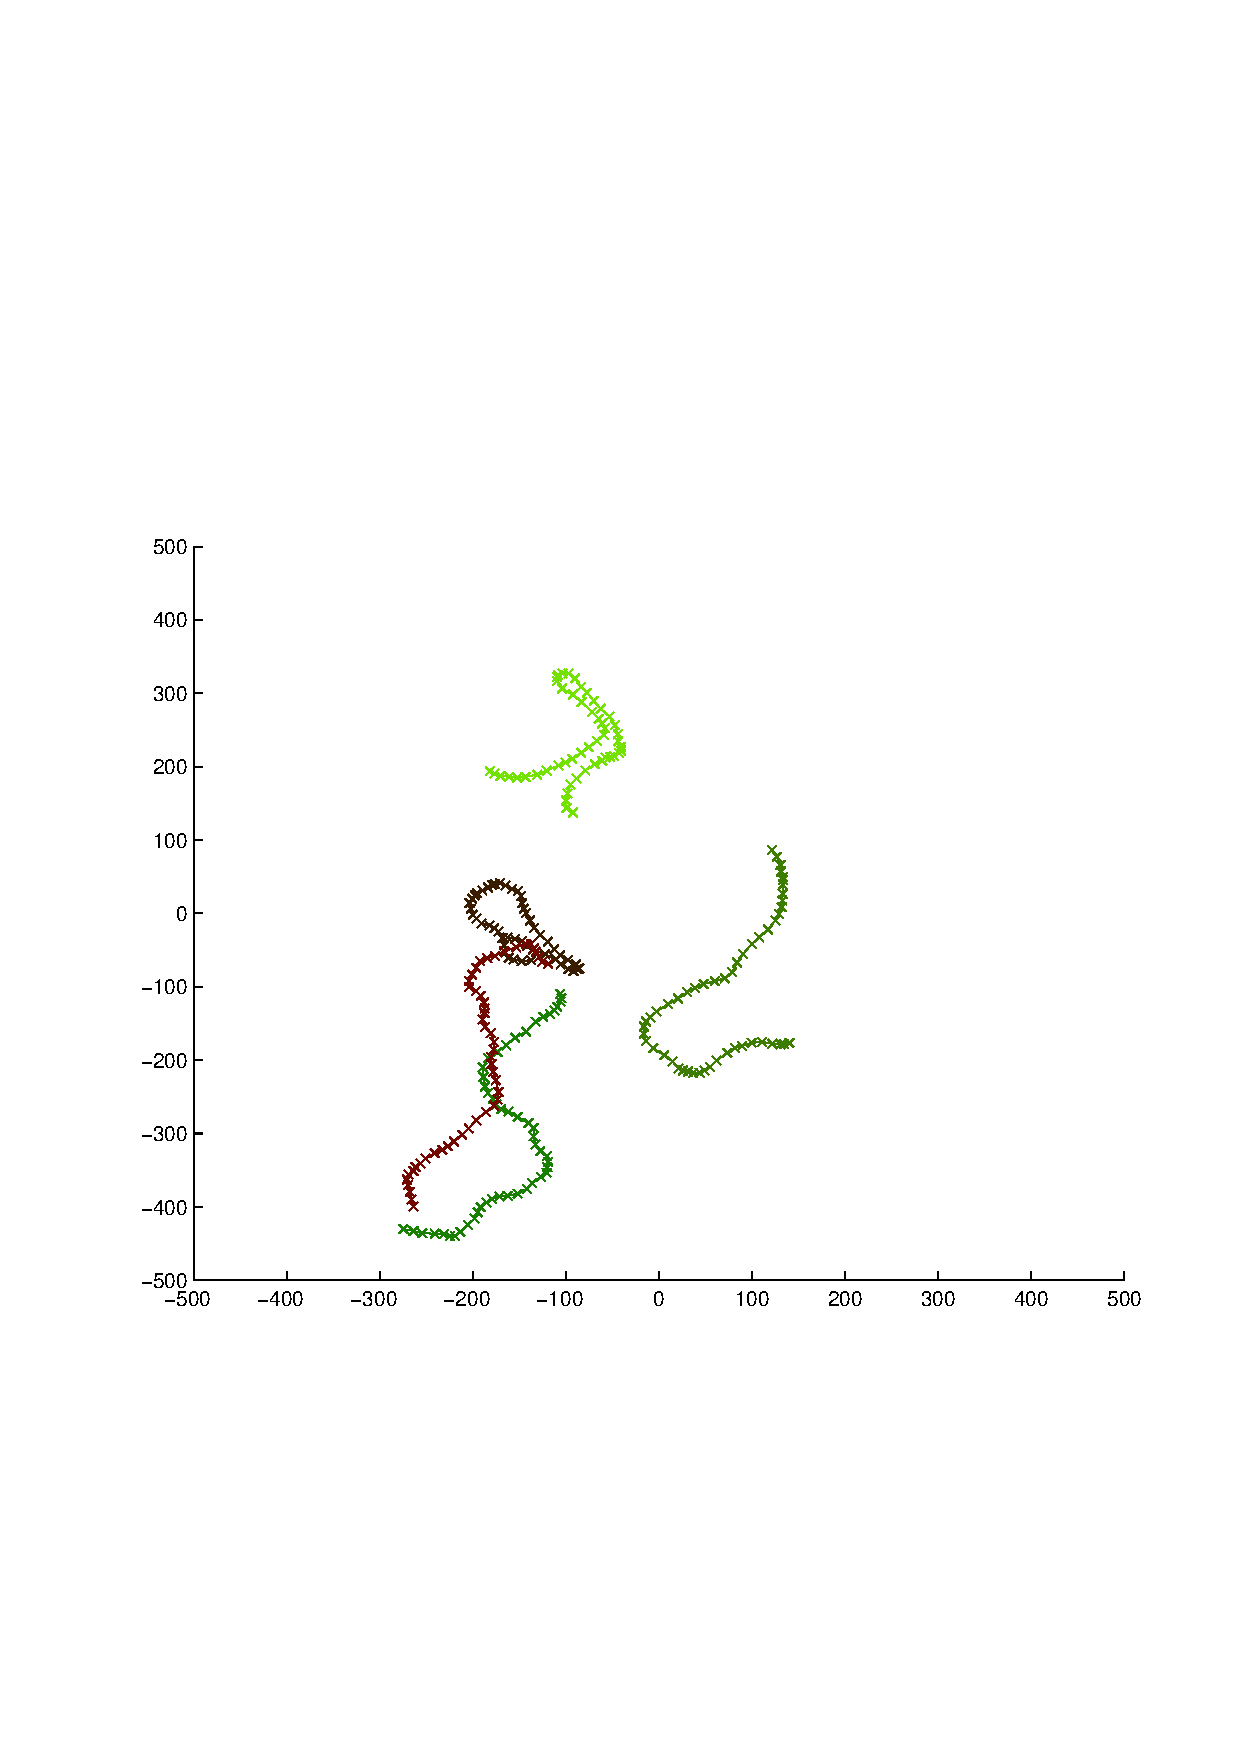
\includegraphics[width=0.3\columnwidth]{results_wide_noise_state.pdf}}
\subfigure[linear observations]{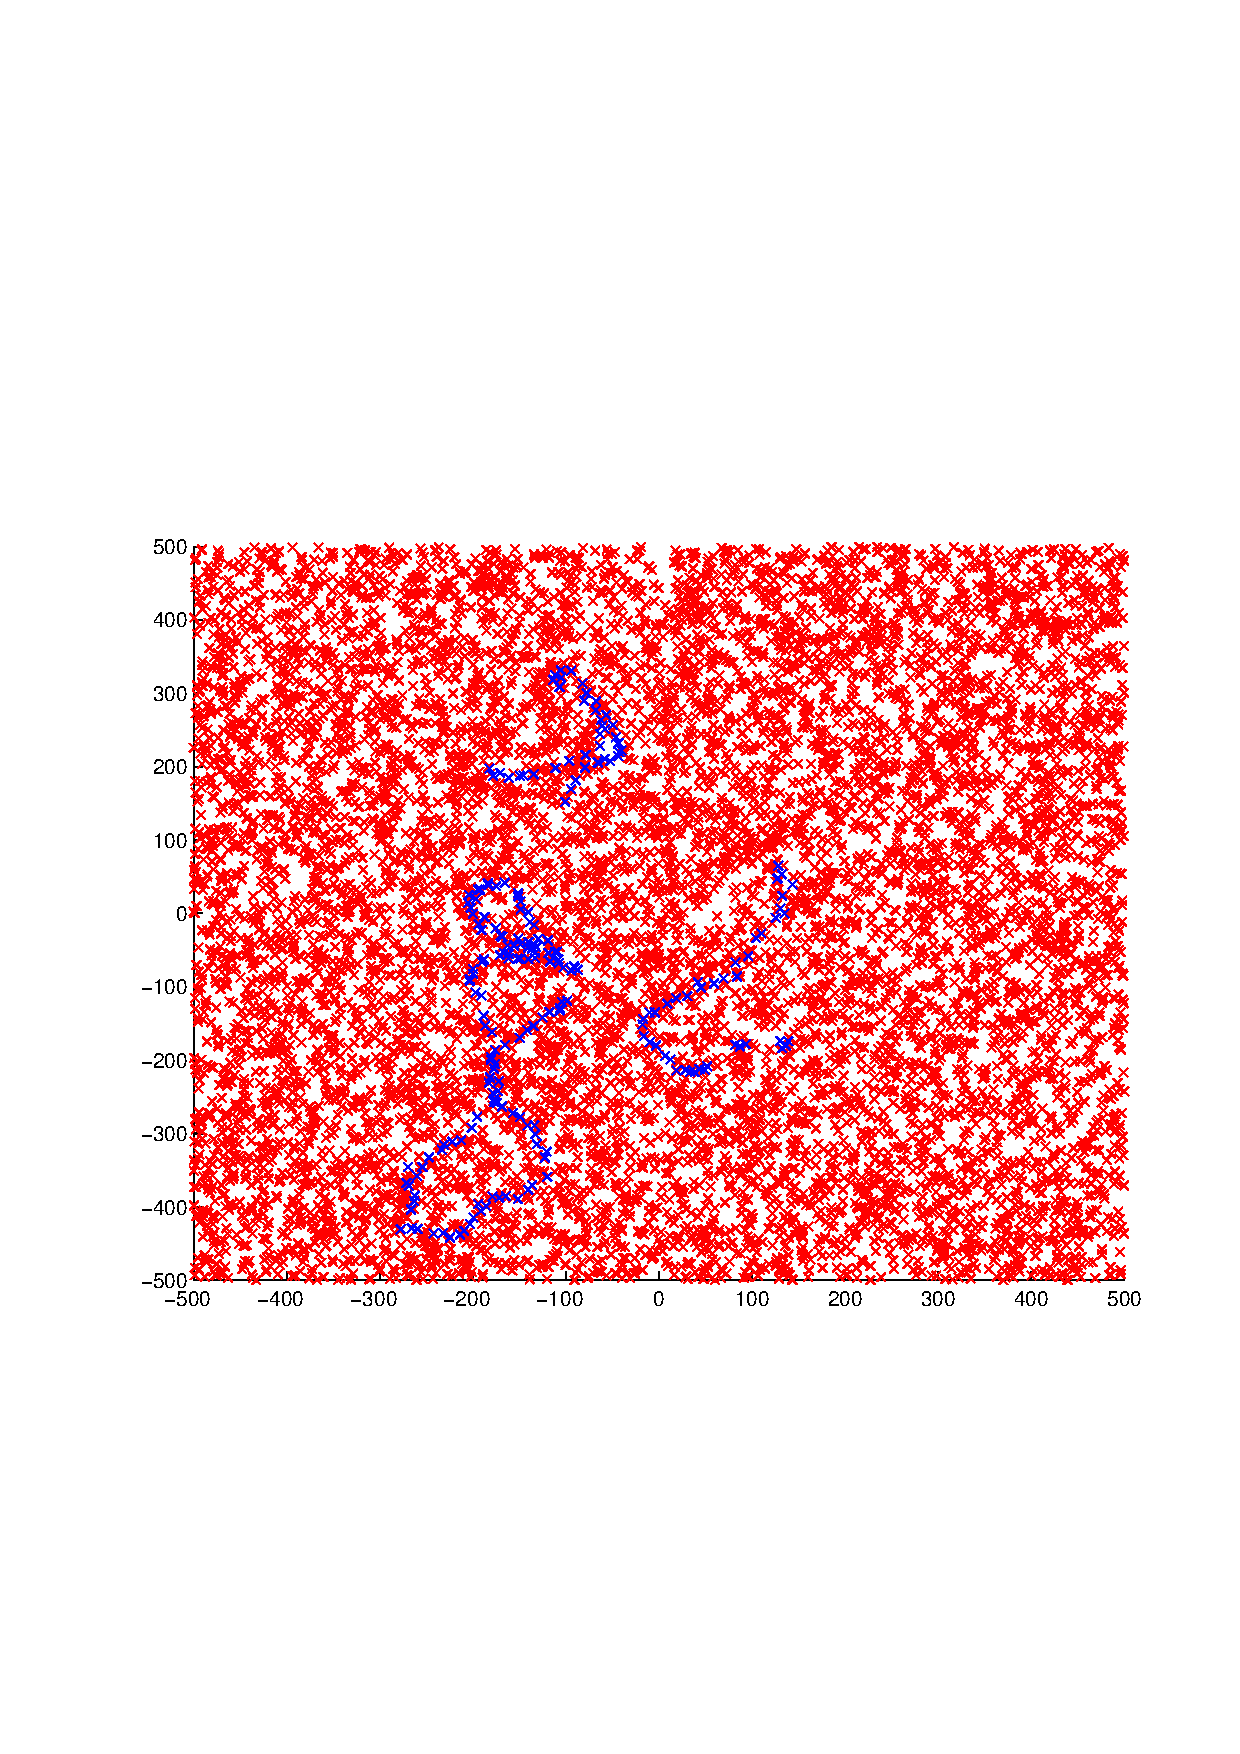
\includegraphics[width=0.3\columnwidth]{results_wide_noise_lGobs.pdf}}
\subfigure[bearing-range observations]{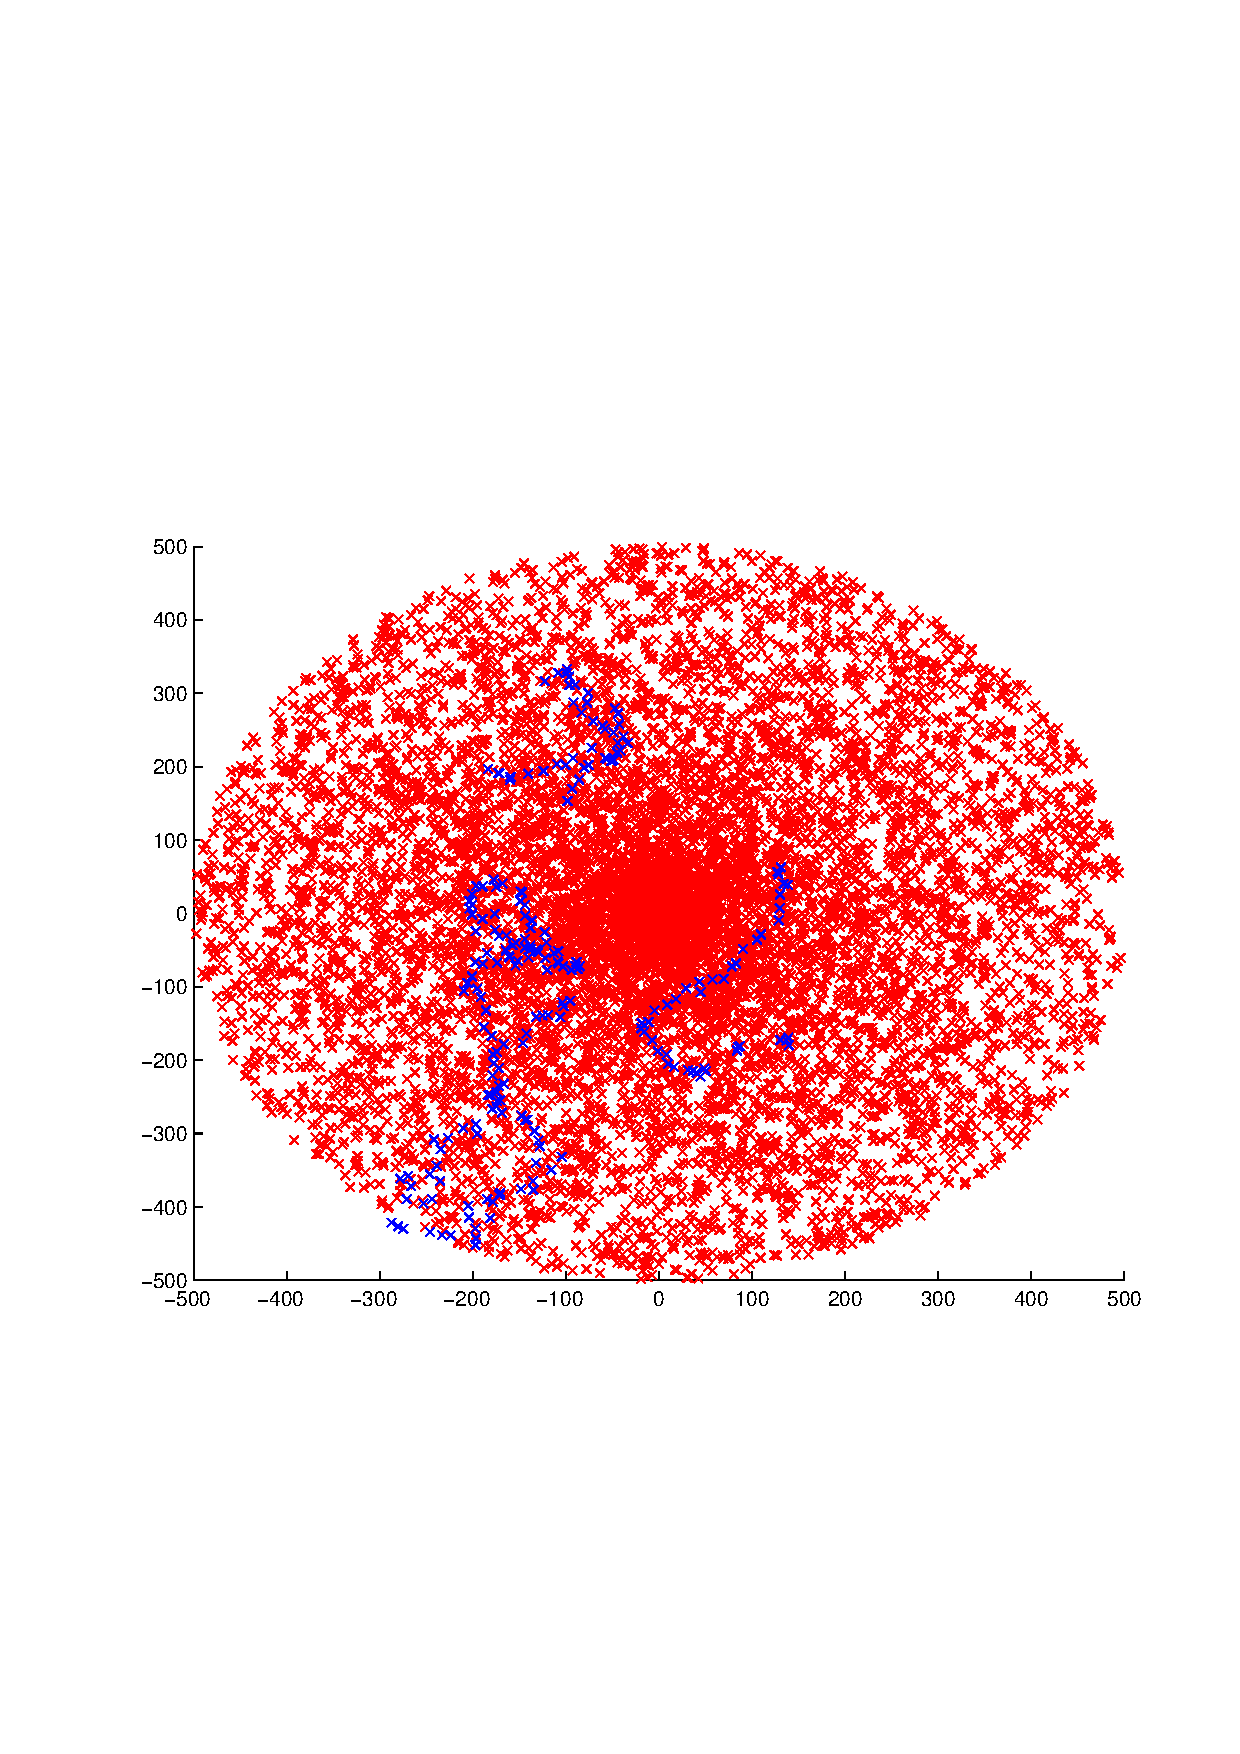
\includegraphics[width=0.3\columnwidth]{results_wide_noise_brobs.pdf}}
\caption{Case 3}%
\label{fig:EgScen3}%
\end{figure}
\begin{figure}%
\subfigure[state]{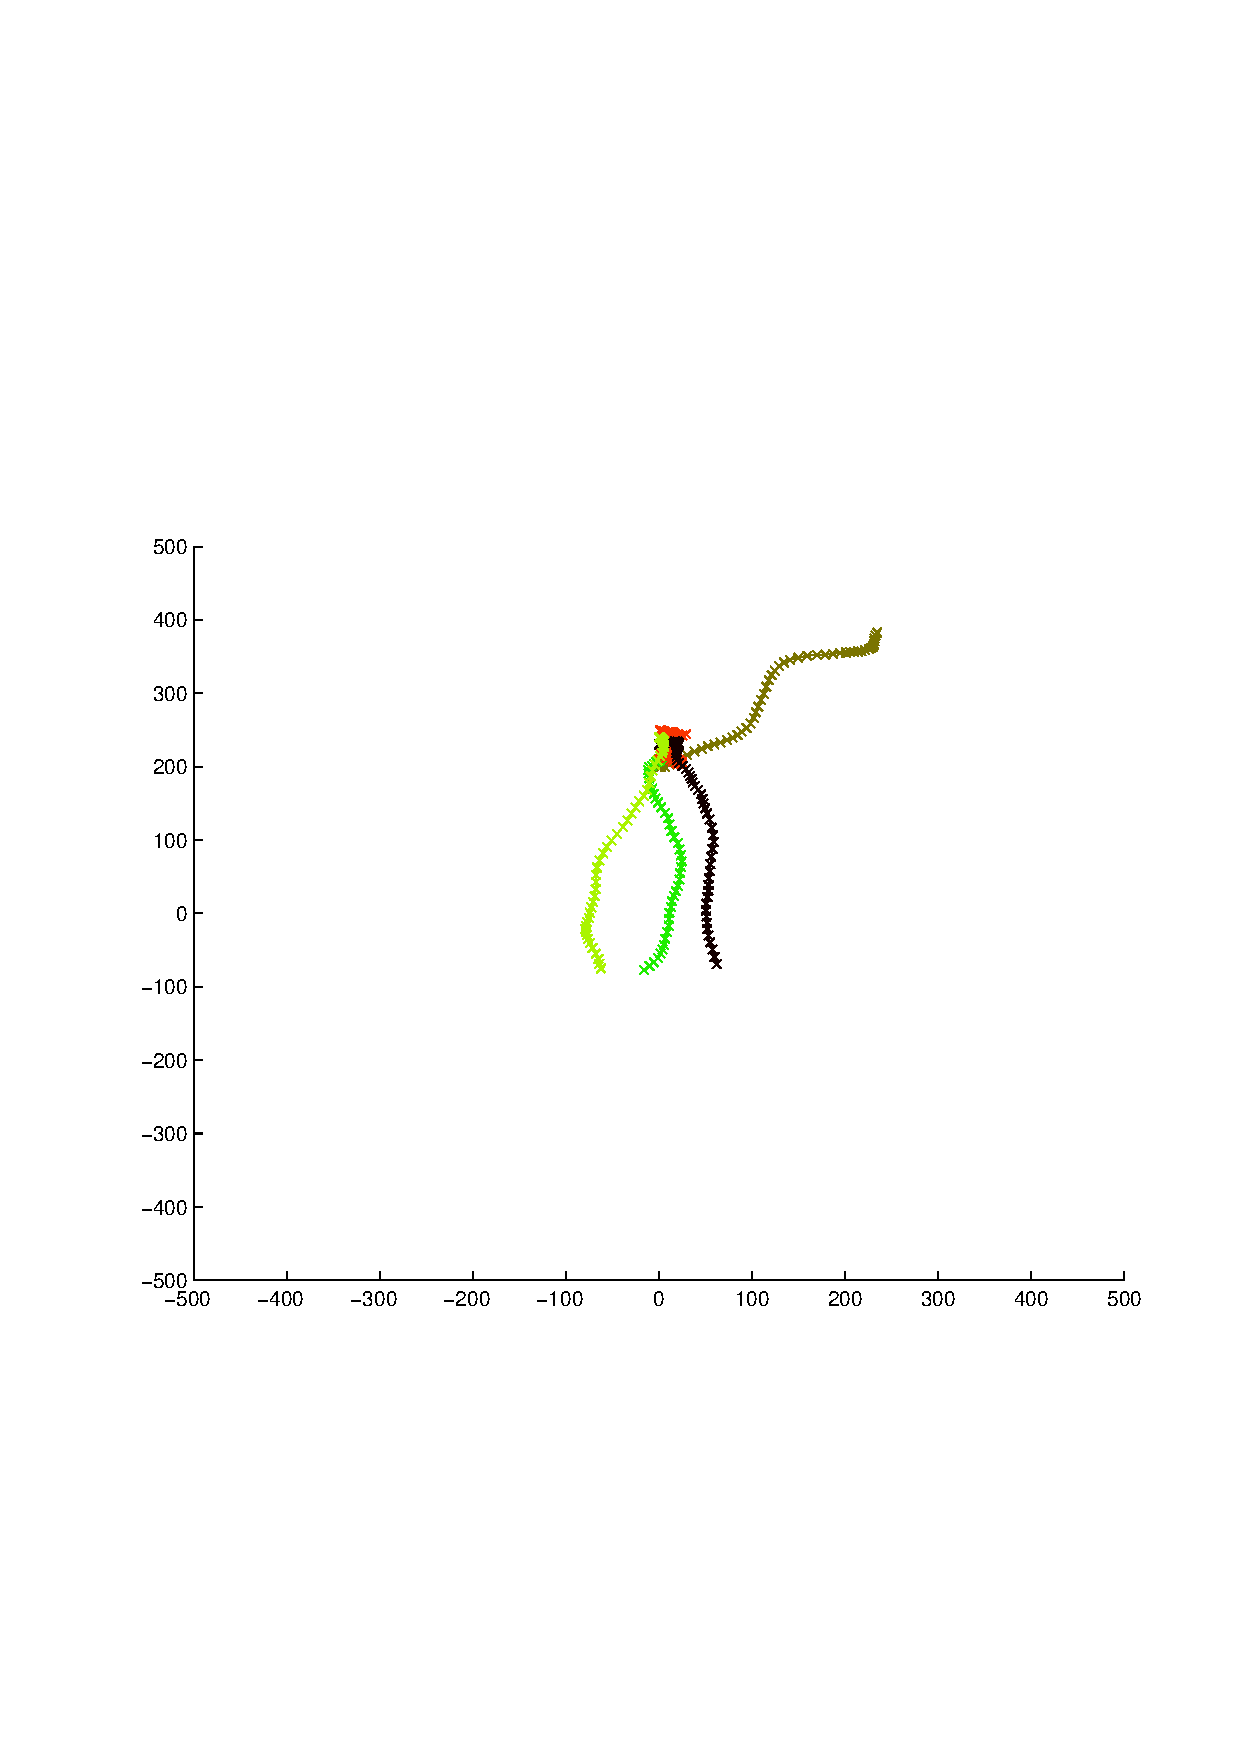
\includegraphics[width=0.3\columnwidth]{results_close_state.pdf}}
\subfigure[linear observations]{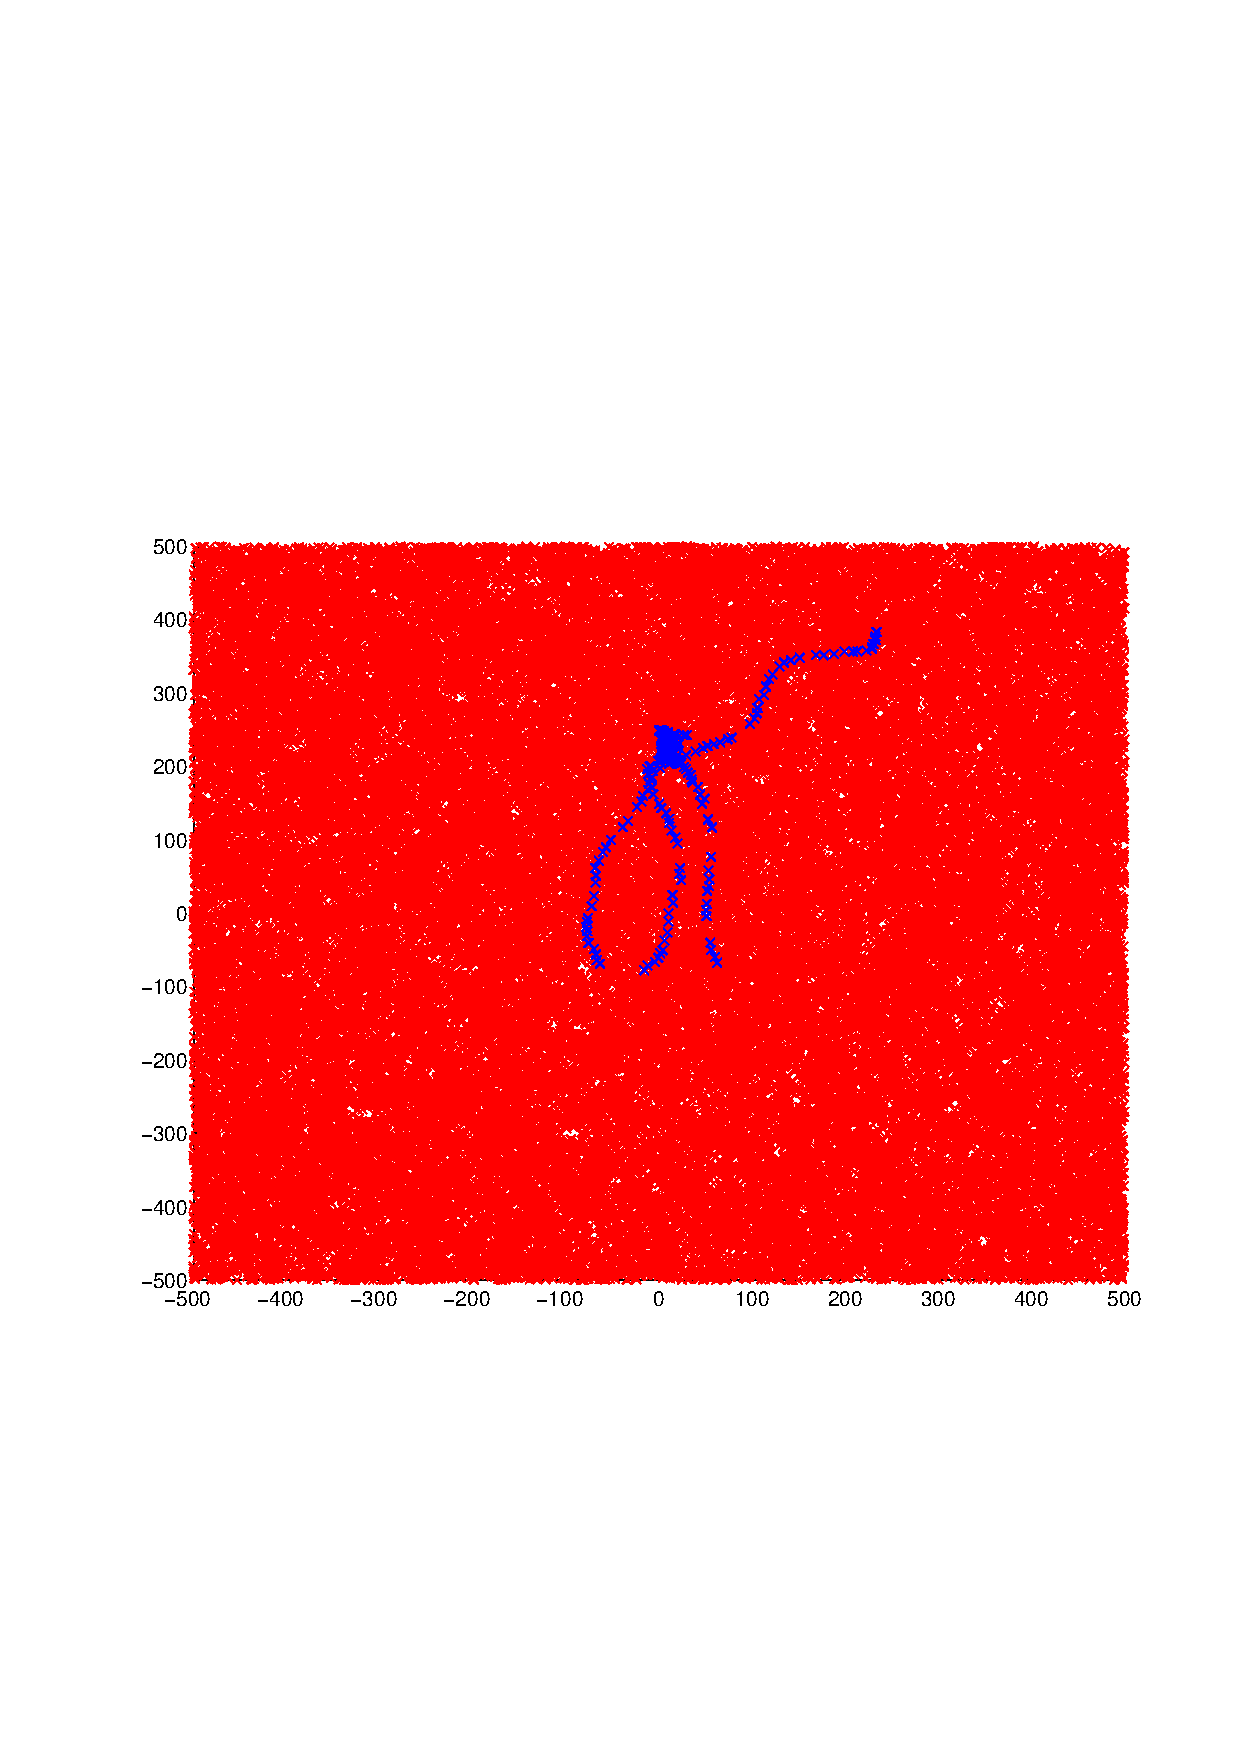
\includegraphics[width=0.3\columnwidth]{results_close_lGobs.pdf}}
\subfigure[bearing-range observations]{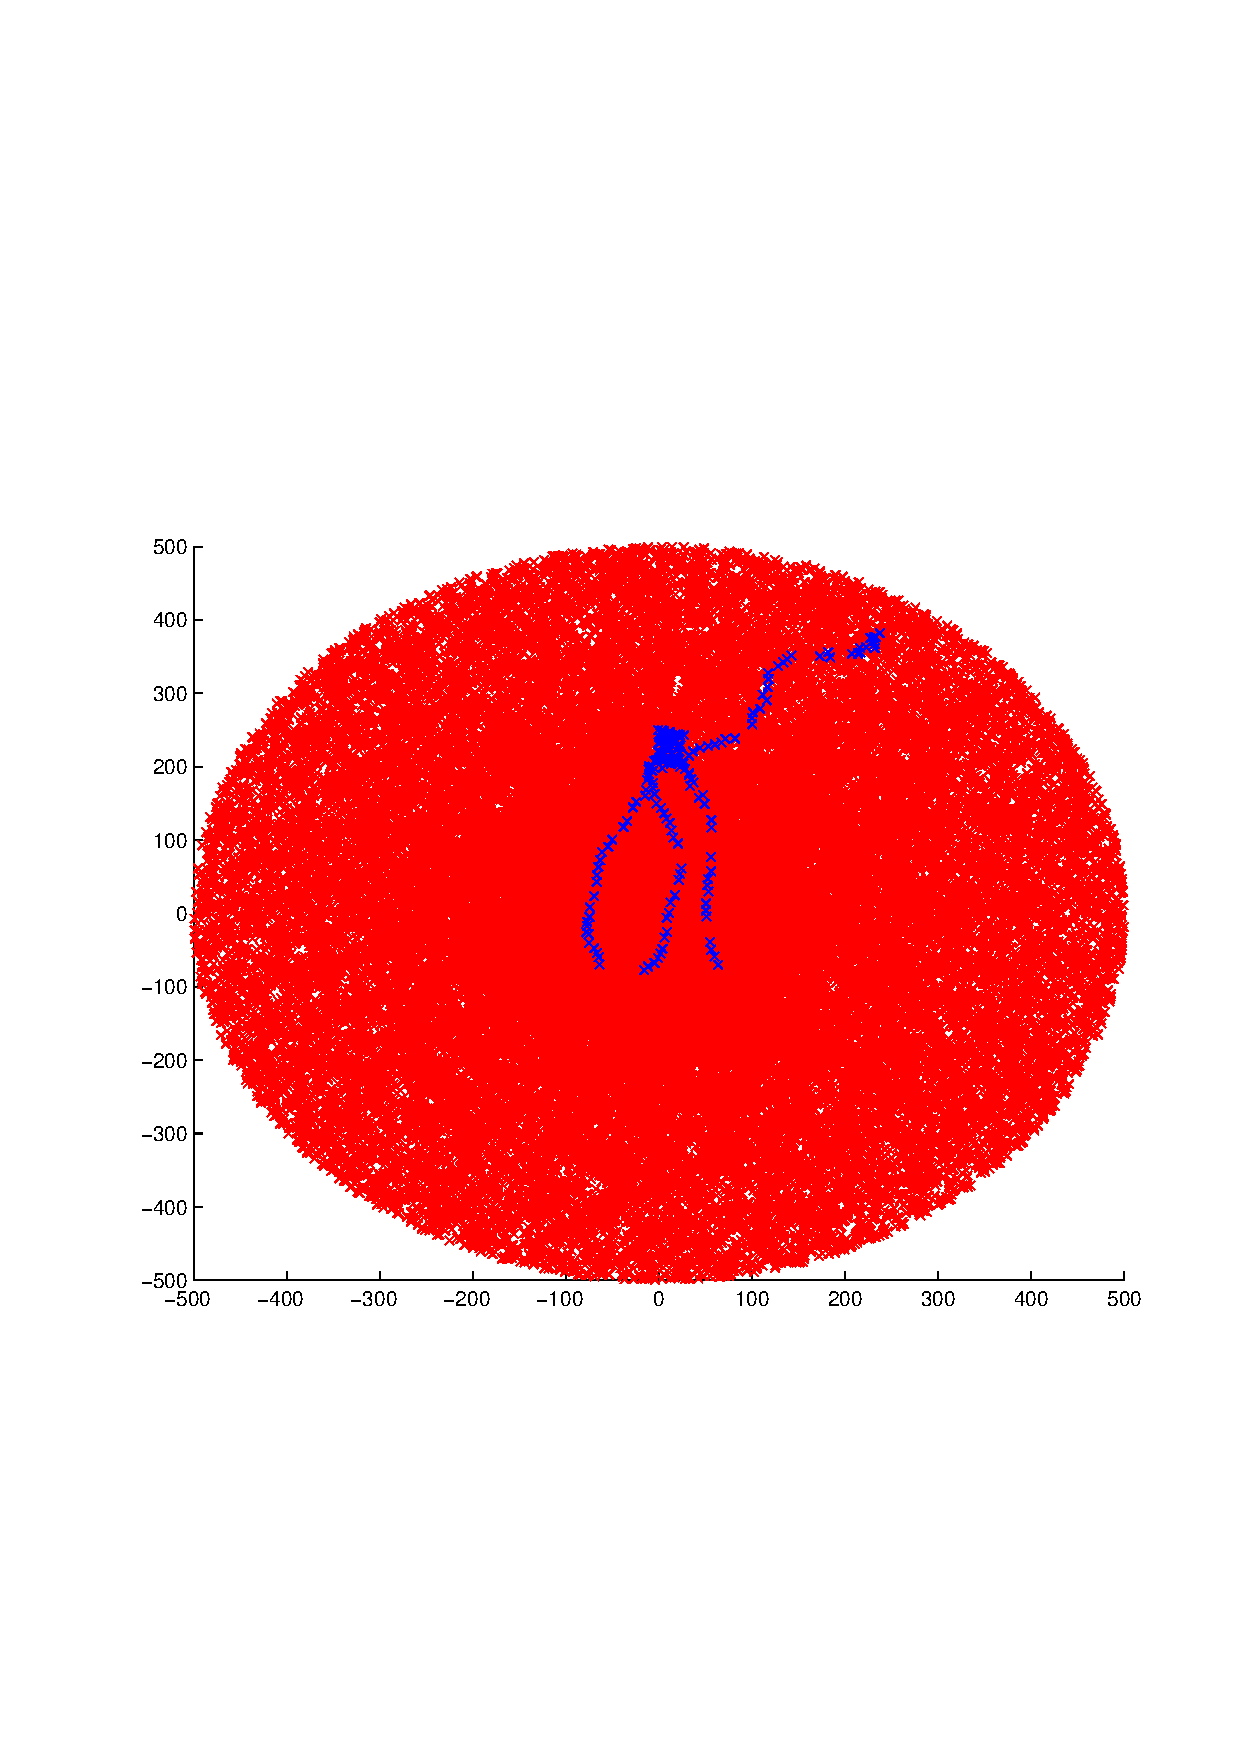
\includegraphics[width=0.3\columnwidth]{results_close_brobs.pdf}}
\caption{Case 4}%
\label{fig:EgScen4}%
\end{figure}

Each scene is $1000 \times 1000$. The velocity of the targets is limited to 10. The period between time steps is 1. The case-specific parameters used are shown in table~\ref{tab:CaseParameters}

\begin{table}%
\begin{center}
\begin{tabular}{|c|c|c|c|c|}
\hline
 & case 1 & case 2 & case 3 & case 4 \\
\hline \hline
process variance & 1 & 1 & 10 & 1 \\
observation variance (linear) & 1 & 1 & 10 & 1 \\
bearing variance (nonlinear) & $10^{-4}$ & $10^{-4}$ & $10^{-3}$ & $10^{-4}$ \\
range variance (nonlinear) & 1 & 1 & 10 & 1 \\
expected no. clutter ($\mu_C$) & 200 & 1000 & 200 & 1000 \\
detection probability ($P_D$) & 0.9 & 0.75 & 0.9 & 0.75 \\
\hline
\end{tabular}
\end{center}
\caption{}
\label{tab:CaseParameters}
\end{table}

The SISR algorithm was run with 500 particles per target. The MCMC algorithm used 5000 iterations and updated the targets in a deterministic order. All algorithms employed gating at 5 standard deviations using a normal approximation.